%Når du starter på en opgave skriver du \begin{opgave}{navnet på opgaven}{sværhedsgrad}, hvor sværhedsgraden skrives som 1,2 eller 3, hvor 3 er den sværeste. 
%Når opgaven er slut skrives \end{opgave}. 
%Såfremt der er delopgaver skrives delopgaver som \opg 

%Eksempel på opgave 
%\begin{opgave}{Polære koordinater}{1}
  %Den kinetiske energi af et legeme, der bevæger sig i 2D-planet er
  %i kartesiske koordinater ($x$ og $y$) givet ved ligning
  %(1.11).
  %
  %\opg Beregn $\dt{x}$ og $\dt{y}$ i polære koordinater og vis
  %derefter, at den kinetiske energi udtrykt i polære koordinater er
  %givet ved ligning (1.12).
%\end{opgave}

\chapter{Laserfysik Opgaver}

Rettelser til kompendiet: I ligning 2.40, 2.41 og i det første led i ligning 2.43 skal $L$ i nævneren slettes! 

\begin{opgave}{Lasere med Forskellige Farver}{1}
Forestil dig at have to lasere, hvor den enes lys er rødt og den andens er grønt. 
\opg Hvad er forskellen mellem de atomer, der bruges til at genere hhv. rødt og grønt lys?
\opg Hvilken af de to har den højeste frekvens?
\end{opgave}

\begin{opgave}{Partikel--Bølge--Dualitet}{2}
Man kan i et meget simpelt forsøg vise at lys også har bølgeegenskaber som en konsekvens af partikel--bølge--dualiteten. Eksperimentet hedder \emph{dobbeltspalte eksperimentet}, og I har måske hørt om det før. I eksperimentet bruger man en plade med to spalter, hvorpå man lyser med en lyskilde (f.eks. en laser). Man ser at lyset efter pladen har spredt sig ud i forskellige ordner, man ser altså en række af lysprikker, et såkaldt inteferensmønster. 
% som man kunne forestille sig skulle komme fra de to spalter. Det skyldes, at lyset har bølgeegenskaber, og derfor udbreder sig som bølger. Bølgerne intefererer med hinanden, således at der dannes konstruktiv og destruktiv inteferens, der giver et inteferensmønster af lysprikker.  
\opg Hvorfor giver lysets bølgeegenskaber anledning til et inteferensmønster?
\opg Hvordan vil du forvente at lyset ser ud på en væg efter det har været gennem pladen, hvis lyset kun har partikelegenskaber? 
\end{opgave}

\begin{opgave}{Populationinversion}{2}
Som beskrevet i Laserfysik skal vi opnå populationinversion i lasersystemet, hvor størstedelen af atomerne befinder sig i en exiceret tilstand fremfor i grundtilstanden, således at stimuleret emission kan dominere. 
\opg Overbevis dig selv om, at de processerne stimuleret absorption og stimuleret emission er de inverse af hinanden (den modsatte proces)
\opg Hvorfor kan man så ikke bruge et 2--niveau system for at lave en laser?
\end{opgave}

\begin{opgave}{Verdens Første Laser - Rubin Laseren}{3}
En rubinlaser -- verdens første laser -- er en krystallaser, som pumpes af en blitzlampe udenom krystallen. Krystallen består af aluminiumoxid ($\text{Al}_2\text{O}_3$), hvori der er tilsat en meget lille mængde krom-ioner ($\text{Cr}^{3+}$).
\begin{figure}[h!]
  \centering
  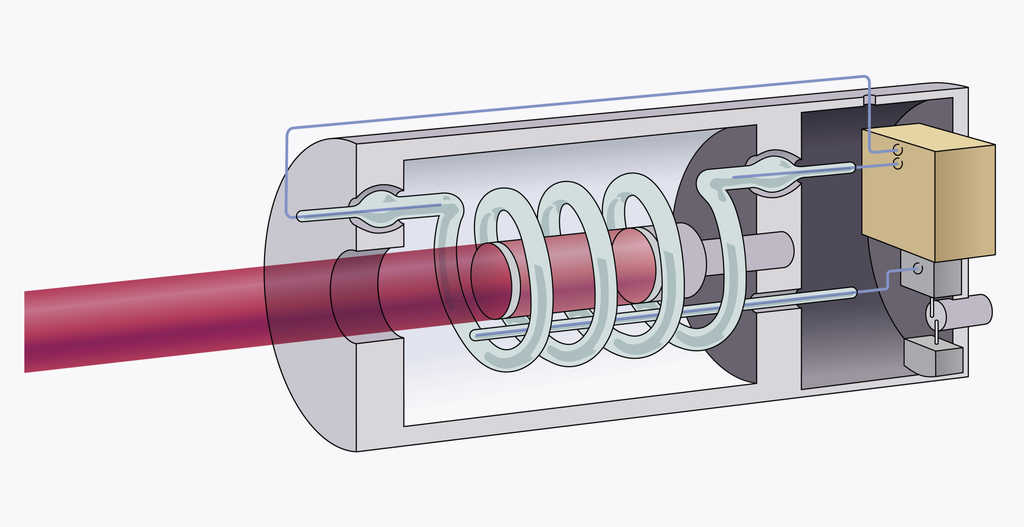
\includegraphics[width=0.6\textwidth]{Laserfysik/rubin_laser_diagram.jpg}
  \caption{Skematisk tegning af en rubin-laser}
  \label{fig:rubin_diagram}
\end{figure}
 Det er overgange i $\text{Cr}^{3+}$, som udsender laserens røde lys.
\opg Overvej, hvorfor lampen er formet som en spiral rundt om krystallen (se figur \ref{fig:rubin_diagram}).
\opg Figur \ref{fig:rubin_energi_diagram} viser de relevante energi-niveauer for $\text{Cr}^{3+}$. Fotonerne fra blitzlampen pumper atomerne op i de højere energiniveauer $E_3$ og $E_4$, som henfalder til to niveauer, som ligger meget tæt på hinanden, samlet kaldet $E_2$. Levetiden af $E_2$-niveauet er længere end levetiden af atomet i $E_3$ og $E_4$, så antallet at atomer i $E_2$ kan blive højere end i de andre niveauer, inklusiv grundtilstanden pga. pumpningen fra blitzlampen. Derfor kan der udsendes fotoner ved hjælp af stimuleret emission fra $E_2$, som udsendes med to røde bølgelængder (se Figur \ref{fig:rubin_energi_diagram}). 
\begin{figure}[h!]
  \centering
  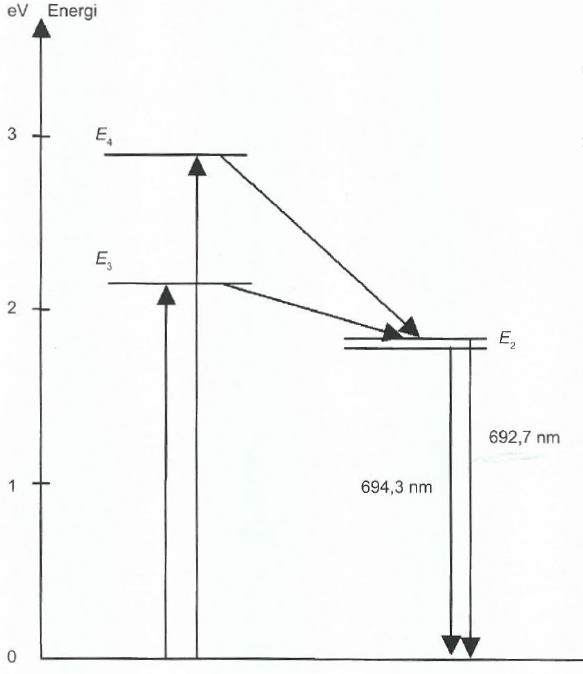
\includegraphics[width=0.5\textwidth]{Laserfysik/rubin_energi}
  \caption{De relevante energi-niveauer i $\text{Cr}^{3+}$.}
  \label{fig:rubin_energi_diagram}
\end{figure}
Hvilken energi bærer laserens udsendte fotoner (ca.)?

\emph{svar: $\approx 2,9\cdot 10^{-19} \joule$}
\opg En lasers rubinkrystal har form som en cylinder med længde $L=6\centi\meter$ og diameter $D=0,5\centi\meter$. I krystallen er $0,035\%$ af aluminiumatomerne udskiftet med $\text{Cr}^{3+}$. Hvor mange $\text{Cr}^{3+}$-atomer findes i krystallen? Du skal bruge følgende oplysninger: tætheden af aluminium er $\rho_\text{Al}=2,7\g/\cm^3$, den molære vægt af aluminium er $M_\text{Al}=27\g/\mol$ og man relaterer antallet af atomer per mol af et stof gennem Avogadros tal: $R_A = 6,022 \cdot 10^{23} \mol^{-1}$. \emph{Hint: find først antal aluminiumatomer indeholdt i cylinderens volumen}.

\emph{svar: $\approx 2,5 \cdot 10^{19}$} 
\opg En rubinlaser bliver ofte for varm til at udsende lys kontinuert, og udsender derfor i stedet lyset i pulser. Forestil dig, at alle $\text{Cr}^{3+}$-atomerne i laseren fra sidste delopgave (se svaret nederst i opgaven) er pumpet så de nu befinder sig i $E_2$, hvorefter laseren udsender alle fotoner med én puls med varighed $2,5 \cdot 10^{-6}\s$. Hvad er effekten af én laserpuls?
\opg En rubinlaser har ingen spejle, men krystallens ender er slebet for at kunne reflektere fotonerne og skabe stående bølger. Hvor mange hele antal bølgelængder svarer længden $L \approx 6\centi\meter$ af en rubinkrystal til for laserlys med $\lambda = 694,4 \cdot 10^{-9} \m$?. Hvor mange knudepunkter opstår i de stående bølger?
\opg Kan du forestille dig, hvorfor det er vigtigt at holde en laser ved stabil temperatur?
\end{opgave}

\begin{opgave}{Approksimation af Gevinstkoefficient}{2}
Denne opgave kræver brug af opgave 8 fra matematik opgaverne. \\
Såfremt reflektiviteten af spejlene i en laserkavitet er stor, dvs. $r_1r_2>0,9$ kan gevinstkoefficienten $g(\nu)$ (ligning 2.20) approksimeres til ligning 2.21. 
\opg Beregn hvordan ligning 2.20 approksimeres til ligning 2.21. \emph{Hint: antag $r_1r_2\approx 1-x$ og sæt $a=0$.}
\end{opgave}

\begin{opgave}{Flere--Niveau systemer}{2}
I Laserfysik er et 3-- og 4--niveau lasersystem præsenteret. Det gives at pumperaten ved tærskelværdien for systemerne er hhv. 
\begin{equation}
(P_t)_3 = \frac{N_T+\Delta N_t}{N_T - \Delta N_t}\Gamma_{21} \,\,\,\,\,\, \text{og} \,\,\,\,\,\, (P_t)_4 = \frac{\Delta N_t}{N_T - \Delta N_t}\Gamma_{21},
\end{equation}
hvor $N_T$ er den totale population og $\Delta N_t$ er $N_2-N_1$ ved tærskelværdien. 
\opg Hvilket system kræver mindst pumpning? Og hvorfor ser vi på pumperaterne ved tærskelværdien? 
\opg Hvilket system ville du foretrække? Hvorfor? 
\end{opgave}

\begin{opgave}{Kavitet}{1}
Et medium har en længde på 10 cm og en gevinstkoefficient på $0,025$cm$^-1$. To spejle med samme reflektivitet placeres i enderne af mediet. Vi antager at tabene ved spejlene pga. absorption og spredning er så små, at de kan negligeres. 
\opg Beregn reflektiviteten, der er nødvendig for at lasing kan opnåes. 
\opg Hvad er transmissionskoefficienten? 
\opg Er det optimalt at have to spejle med samme reflektivitet i en laser system? Hvorfor, hvorfor ikke?
\end{opgave}

\begin{opgave}{Foton Output}{2}
En kavitet for en He-Ne laser(632,8 nm) er 50 cm med reflektivitet $r_1=1$ for det ene spejl og $r_2=0,98$ for det andet spejl. Vi antager at tabene er meget små. Effekten (output power) af laseren er $Pwr = 10$ mW. 
\opg Hvor mange fotoner udsendes pr. sekund?
\opg Hvad er antallet af fotoner i kaviteten ved tærskelværdien?
\end{opgave}

\begin{opgave}{Pulserende eller Kontinuert?}{1}
En laser, der bruges til at skære i elementer, som f.eks. plastik har en væsentlig større intensitet end en laserpointer, der bruges i undervisningen (heldigvis!).
\opg Hvis du skulle bygge begge lasere, ville du så lave dem kontinuerte eller pulserende? Hvorfor?
\end{opgave}

\newpage


\chapter{Laserfysik Facitliste}

\begin{opgave}{Lasere med Forskellige Farver}{1}
\opg Atomerne har forskellige overgangsenergier. Bølgelængden afhænger af energien, og da rødt og grønt lys ikke har samme bølgelængde, må overgangsenergierne derfor være forskellige for atomerne, der bruges til at lave hhv. rødt og grønt lys. 
\opg Rød har længere bølgelængde end grøn, og grøn har derfor en større frekvens, da bølgelængde og frekvens er omvendt proportionale. 
\end{opgave}

\begin{opgave}{Partikel--Bølge--Dualitet}{2}
\opg Bølger kan intefere, som vi kender det fra stående bølger på en snor. De kan inteferere konstruktivt eller destruktivt. Ved konstruktiv inteferens vil man se en lysplet, da to bølger ''lægges sammen'', hvor i mod man ved destruktiv inteferens ikke vil se en lys plet, da bølgerne her vil udslukke hinanden. 
\opg Hvis lyset kun har partikelegenskaber kan man tænke på lys som små kugler, og man vil derfor forvente kun at se to lysprikker, der vil opstå pga. de to spalter i pladen. 
\end{opgave}

\begin{opgave}{Populationinversion}{2}
\opg Se på billedet for stimuleret emission. Vend nu processen om, dvs. Elektronen nu ligger i grundtilstanden. I denne omvendte proces kommer der altså to fotoner ind, hvoraf en af dem absorberes af elektronen, således at den hopper op i den exciterede tilstand. Den anden foton fortsætter bare og har ingen effekt. Hvis du nu sætter en ekstra foton ind i billedet for stimuleret absorption er det præcis det samme billede, som lige beskrevet som den omvendte proces af stimuleret emission. 
\opg Da vi nu har argumenteret for, at stimuleret emission og stimuleret absorption er de omvendte processer af hinanden, må de også ske med samme sandsynlighed.  Lige stor sandsynlighed for de to processer betyder at man kan sige at hver gang ét atom exciteres, så henfalder et andet atom. Derfor kan størstedelen af atomerne aldrig være i en exciteret tilstand, og stimuleret emission kan ikke dominere. Derfor kan 2-niveau-systemer ikke bruges til at skabe laserlys med.
\end{opgave}

\begin{opgave}{Verdens Første Laser -- Rubin Laseren}{3}
\opg Hvis lampen er formet rundt om kaviteten, så belyser den fra så mange retninger som muligt, hvilket effektivt kan pumpe systemet.
\opg På figuren ses det, at de udsendte fotoner har bølgelængderne $\lambda=692,7\nano\m$ og $\lambda=694,3\nano\m$ ($1\nano\m = 1$ nanometer $= 10^{-9}\m$). Vi tager gennemsnittet af de to for at udregne den gennemsnitlige energi af en foton.
\begin{align}
E_\text{foton} &= h \cdot \frac{c}{\lambda} \\
&= h \frac{c}{\left( 692,7 \cdot 10^{-9} \m + 694,3 \cdot 10^{-9} \m \right)/2} \\
&\approx 2,9 \cdot 10^{-19}\joule 
\end{align}
\opg Hvis man vil finde antal aluminium-atomer i en volumen skal man bruge:
\begin{equation}
\text{\# atomer} = (\rho_\text{Al} \cdot V)/M_\text{Al} \cdot R_A,
\end{equation}
($\rho_\text{Al} \cdot V$ giver antal gram aluminium i cylinderen, og deler man med den molare masse, så ved man hvor mange mol, der findes i cylinderen. Ved at gange med Avogadros tal, $R_A$, så finder man antal atomer). Volumenet af cylinderen er $V=\pi(D/2)^2 \cdot L$. Antal aluminium-atomer er derfor
\begin{equation}
\text{ \# Al-atomer} \approx 7 \cdot 10^{22}.
\end{equation}
Idet vi får at vide at $0,035\%$ af aluminium-atomerne er udskiftet med $\text{Cr}^{3+}$, så finder vi antal Cr-atomer som:
\begin{align}
\# \text{Cr-atomer} &= \#\text{Al-atomer} \cdot \frac{0,035}{100} \\
&\approx 2,5 \cdot 10^{19}.
\end{align}
\opg Effekten er udsendt energi per sekund. Hvis alle Cr-atomerne udsender lys på én gang, så er den samlede puls-energi $E_\text{puls} = E_\text{foton} \cdot \# \text{Cr-atomer}$, hvor vi bruger at vi fandt energien af en foton i delopgave 2. Effekten findes:
\begin{align}
P_\text{puls} &= \frac{E_\text{puls}}{t_\text{puls}} \\
&= \frac{ E_\text{foton} \cdot \# \text{Cr-atomer}}{t_\text{puls}} \\
&= \frac{2,9\cdot 10^{-19}\joule \cdot 2,5 \cdot 10^{19}}{2,5 \cdot 10^{-6}\s} \\
&= 2,9 \mega\watt
\end{align}
\opg For en krystal med længde $L=6\centi\meter$ og $\lambda = 694,4 \cdot 10^{-9} \m$ så er antal bølgelængder ca.
\begin{equation}
\frac{L}{\lambda} = 86406
\end{equation}
Vi ved at der opstår stående bølger i kaviteten, og at der derfor gælder:
\begin{align}
L &= n\frac{\lambda}{2} \\
\rightarrow n &= 2 \frac{L}{\lambda} \\
&= 172812 
\end{align}
Ved f.eks. at kigge på figur 4.3 så ses det, at antal knudepunkter er givet ved $n+1$. Antal knudepunkter er derfor $172813$.
\opg Hvis materialer opvarmes eller nedkøles vil de hhv. udvide og trække sig sammen, hvilket i værste fald kan resultere i, at længden af kaviteten ændres, sådan at der ikke kan opstå stående bølger.
\end{opgave}

\begin{opgave}{Approksimation af Gevinstkoefficient}{2}
\opg Ligningen der skal approksimeres er 
\begin{equation}
g_t = -\frac{1}{2L}\ln(r_1r_2). 
\end{equation}
Vi følger hintet og sætter $r_1r_2 = 1-x$, så 
\begin{equation}
g_t = -\frac{1}{2L}\ln(1-x). 
\end{equation}
Vi ønsker nu at approksimere funktionen med en Taylor udvikling. Vi sætter startsbetingelsen $a=0$ jævnfør hintet, og vi ser kun på de to første led. De andre led kan også beregnes, men de bidrager kun ganske lidt. 
\begin{equation}
f(x) \approx f(0) + x\d{f}{x}_{x=0} = 0 + x\cdot \frac{-1}{1-0} = -x
\end{equation}
$g_t$ bliver derfor 
\begin{equation}
g_t = -\frac{1}{2L}(-(1-r_1r_2)) = \frac{1}{2L}(1-r_1r_2). 
\end{equation}
\end{opgave}

\begin{opgave}{Flere-Niveau Systemer}{2}
\opg Vi ser på forholdet mellem dem for at finde ud af hvilket system, der kræver mindst pumpning. 
\begin{equation}
\frac{(P_t)_4}{(P_t)_3} = \frac{\Delta N_t}{N_T + \Delta N_t}.
\end{equation}
Det totale antal af atomer i systemet må være større end populationinversionen, så 
\begin{equation}
(P_t)_4 << (P_t)_3.
\end{equation}
For at opnå lasing kræver et 3 system mere pumpning end et 4 system. 
Vi ser på pumperaterne ved tærskelværdien fordi det lige akkurat er ved denne at lasing kan opnåes. 
\opg Med et 4 system kan vi opnå lasing med en lavere pumperate, og det er derfor at foretrække. 
\end{opgave}

\begin{opgave}{Kavitet}{1}
\opg Da man på forhånd ikke ved om spejlene opfylder $r_1r_2>0,9$ er det ikke gangbart at bruge den approksimerede version af $g_t$. Vi skal altså bruge 
\begin{equation}
g_t = -\frac{1}{2l}\ln(r_1r_2). 
\end{equation}
Da reflektiviteterne antages at være ens, kan vi sætte $r_1r_2=r^2$, som derefter isoleres. 
\begin{align}
g_t &= -\frac{1}{2l}\ln(r^2) 
\Rightarrow\\ -2lg_t &=\ln(r^2) 
\Rightarrow\\ e^{-2lg_t} &=r^2
\Rightarrow\\ r&=\sqrt{e^{-2lg_t}}
\end{align}
Indsættes tallene fås nu
\begin{equation}
r=\sqrt{e^{-2lg_t}} = \sqrt{e^{-2\cdot10\,\text{cm}\cdot0,025\,\text{cm}^{-1}}} = 0,778
\end{equation}
\opg Da $s$ antages at være 0 gælder der $r+t=1$. Transmissionskoefficienten fås da til 
\begin{equation}
r+t=1 \Rightarrow t = 1-r = 1-0,778 = 0,222. 
\end{equation}
Det vil altså sige, at $77,8\%$ af lyset reflekteres og $22,2\%$ transmitteres når lyset rammer et af spejlene. 
\opg Det er ikke optimalt at have to spejle med samme reflektivitet da man kun ønsker, at laserlyset skal komme ud i den ene ende. Derudover kan man heller opnå at $r_1r_2>0,9$ hvis begge reflektviteter er mindre end 1. 
\end{opgave}

\begin{opgave}{Foton Output}{2}
\opg Vi får givet effekten (power) af laserlyset. Effekt har enheden watt, som er defineret som energi pr. tid, dvs. $\text{W} = \frac{\text{J}}{\text{s}}$. Fra dette kan vi se, at det er nødvendigt at dividere med en energi for at få noget pr. sekund. Altså er antallet af udsendte fotoner pr. sekund 
\begin{equation}
\d{q}{t} = \frac{\text{Pwr}}{h\nu},
\end{equation}
hvor $h\nu$ er energien af én foton
\begin{equation}
h\nu = h \frac{c}{\lambda} = 6,626\cdot 10^{-34}\, \text{Js} \, \frac{3\cdot10^{8}\,\text{m/s}}{632,8\cdot 10^{-9}\, \text{m}} = 3,14\cdot 10^{-19}\, \text{J}.
\end{equation}
Vi får så at 
\begin{equation}
\d{q}{t} = \frac{10\cdot10^{-3}\,\text{W}}{3,14\cdot 10^{-19}\,\text{J}} = 3,14\cdot 10^{-16}\, \frac{1}{\text{s}}.
\end{equation}
\opg Vi bruger at 
\begin{equation}
\d{q}{t} = cg(\nu)q, 
\end{equation}
og da vi skal beregen antallet af fotoner ved tærskelværdien er $g(\nu) = g_t$. Vi får da 
\begin{equation}
q = \d{q}{t}\frac{1}{cg_t} = \frac{\text{Pwr}}{h\nu}\frac{1}{cg_t}.
\end{equation}
Da $r_1r_2>0,9$ kan $g_t$ beregnes til 
\begin{equation}
g_t = \frac{1}{2\cdot 0,5 \, \text{m}}(1-0,98) = 0,02\, \text{m}^{-1}. 
\end{equation}
Antallet af fotoner bliver så 
\begin{equation}
q = 3,14\cdot 10^{-16}\, \frac{1}{\text{s}}\, \frac{1}{3\cdot 10^{8} \text{m/s}\cdot 0,02 \, \text{m}^{-1}} = 5,2\cdot 10^9
\end{equation}
\end{opgave}

\begin{opgave}{Pulserende eller Kontinuert}{1}
\opg En pulserende laser pumpes oftest hårdere fordi det kræver mere at opnå populationinversion pga. alle tabene. En kontinuert laser pumpes ikke nær så hårdt da lasersystemet ikke lider af så store tab, som en pulserende laser gør. En større pumpning giver anledning til mere stimuleret emission, der så giver anledning til mere intenst lys. Intensiteten af en pulserende laser er derfor typisk større, da et sådant lasersystem pumpes hårdere. 
\end{opgave}


